%%% lecture 08 %%%
\documentclass{beamer}
\usepackage[utf8]{inputenc}
\usepackage{algorithm2e, amsmath, amssymb, amsfonts, graphicx}
% allow section.equation numbering
\numberwithin{equation}{section}
% use boadilla theme
\usetheme{Boadilla}
% remove navigation symbols
\usenavigationsymbolstemplate{}
% get numbered figure captions
\setbeamertemplate{caption}[numbered]
% changes itemize to circle + other things
\useoutertheme{split}
\useinnertheme{circles}

% command for the title string. change for each lecture
\newcommand{\lecturetitle}{Support Vector Machines}
% allow automatic alert-highlighted references and hyperlinks
\newcommand{\aref}[1]{\alert{\ref{#1}}}
\newcommand{\ahref}[2]{\href{#1}{\alert{#2}}}
% title page stuff. brackets content displayed in footer bar
\title[\lecturetitle]{\lecturetitle}
% metadata. content in brackets is displayed in footer bar
\author[Derek Huang (BAC Advanced Team)]{Derek Huang}
\institute{BAC Advanced Team}
\date{August 14, 2021}

% change "ball" bullet to numbered bullet and section title for section
\setbeamertemplate{section in toc}{\inserttocsectionnumber.~\inserttocsection}
% change ball to gray square (copied from stackoverflow; \par needed for break)
\setbeamertemplate{subsection in toc}{        
    \hspace{1.2em}{\color{gray}\rule[0.3ex]{3pt}{3pt}}~\inserttocsubsection\par
}
% use default enumeration scheme
\setbeamertemplate{enumerate items}[default]
% required line that fixes the problem of \mathbf, \bf not working in beamer
% for later (post-2019) TeX Live installations. see the issue on GitHub:
% https://github.com/josephwright/beamer/issues/630
\DeclareFontShape{OT1}{cmss}{b}{n}{<->ssub * cmss/bx/n}{}

\begin{document}

% title slide
\begin{frame}
    \titlepage
    \centering
    % relative path may need to be updated depending on .tex file location
    
\includegraphics[scale=0.1]{../bac_logo1.png}
\end{frame}

% table of contents slide
\begin{frame}{Overview}
    \tableofcontents
\end{frame}


\section{Linear SVMs}

\subsection{Maximum margin hyperplanes}

\begin{frame}{Motivation}
    \begin{itemize}
        \item
        We saw that logistic regression, LDA/QDA, and na\"{i}ve Bayes
        provide probabilistic models of [class-]conditional distributions.

        \item
        Suppose we have disjoint convex sets $ A, B \subset \mathbb{R}^d $.
        There are several ways to draw a distribution-free ``line''
        (hyperplane) between them.

        \item
        Intuitively, the optimal hyperplane is furthest away from both
        $ A, B $. How can solve the resulting optimization problem?

        \item
        How do we define ``furthest away'' in this context?
    \end{itemize}
\end{frame}

\begin{frame}{Maximum margin hyperplanes}
    \begin{itemize}
        \item
        \textit{Definition.} A \textit{hyperplane} in $ \mathbb{R}^d $ with
        \textit{normal vector} $ \mathbf{a} \in \mathbb{R}^d $ is the affine
        set
        $ \{\mathbf{x} \in \mathbb{R}^d : \mathbf{a}^\top\mathbf{x} = b \} $,
        where $ \mathbf{a} \ne \mathbf{0} $, $ b \in \mathbb{R} $
        \cite{bv_convex_opt}.

        \item
        A hyperplane is the solution set for a nontrivial linear equation with
        a \textit{normal vector} $ \mathbf{a} $, which in 2D is orthogonal
        to the plane.

        \begin{figure}
            \centering
            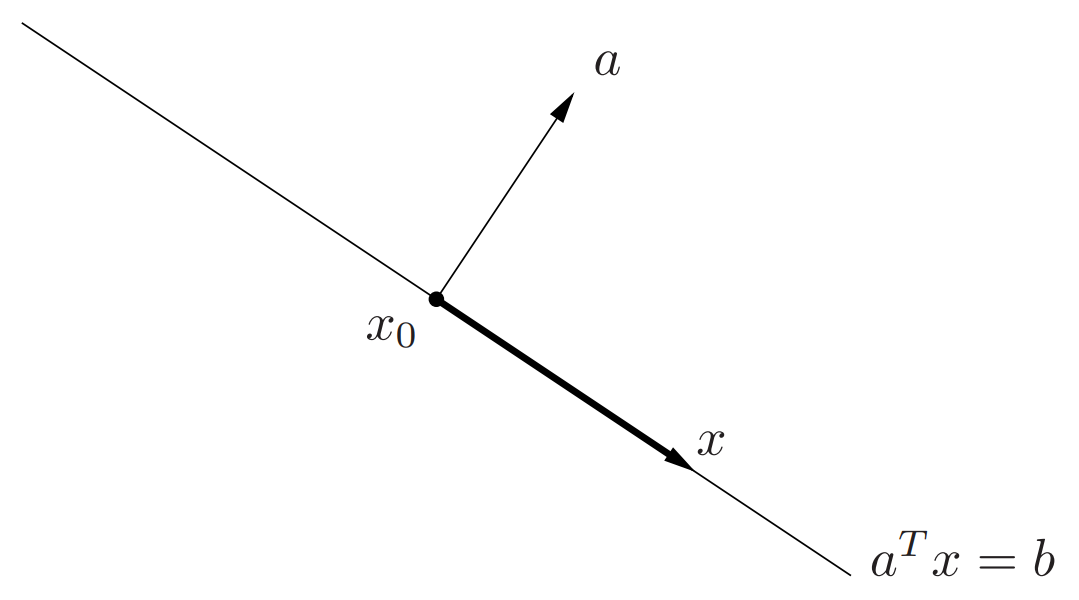
\includegraphics[scale=0.2]{hyperplane.png}
            \vspace{-5 pt}
            \caption{
                A hyperplane with normal vector $ \mathbf{a} \in
                \mathbb{R}^2 $. Note $ \mathbf{a}^\top(\mathbf{x} -
                \mathbf{x}_0) = 0 $\footnote{
                    Figure 2.6 from Boyd and Vandenberghe's
                    \textit{Convex Optimization}.                
                }.
            }
            \label{fig:hyperplane}
            \vspace{-5 pt}
        \end{figure}

        \item
        As seen in Figure \aref{fig:hyperplane}, for hyperplane
        $ L \triangleq \{\mathbf{x} \in \mathbb{R}^d :
        \mathbf{a}^\top\mathbf{x} = b \} $,
        $ \forall \mathbf{x}, \mathbf{y} \in L $,
        $ \mathbf{a}^\top(\mathbf{x} - \mathbf{y}) = 0 \Rightarrow \mathbf{a} $
        is orthogonal to vectors parallel to $ L $.
    \end{itemize}

    % spacing for footnote
    \medskip
\end{frame}

\begin{frame}{Maximum margin hyperplanes}
    \begin{itemize}
        \item
        \textit{Definition.} A \textit{closed halfspace} in $ \mathbb{R}^d $
        with normal vector $ \mathbf{a} \in \mathbb{R}^d $ is a set of the form
        $ \{\mathbf{x} \in \mathbb{R}^d : \mathbf{a}^\top\mathbf{x} \le b\} $
        or $ \{\mathbf{x} \in \mathbb{R}^d : \mathbf{a}^\top\mathbf{x} \ge
        b\} $ \cite{bv_convex_opt}. If we use strict inequalities, the sets
        are \textit{open halfspaces}.

        \item
        By setting $ b $ to $ -b $, we can equivalently define hyperplanes
        with $ \mathbf{a}^\top\mathbf{x} + b = 0 $ and closed halfspaces with
        $ \mathbf{a}^\top\mathbf{x} + b \le 0 $,
        $ \mathbf{a}^\top\mathbf{x} + b \ge 0 $.

        \item
        Note that $ \forall \mathbf{x}' \in \mathbb{R}^d $, given hyperplane
        $ L \triangleq \{\mathbf{x} \in \mathbb{R}^d :
        \mathbf{w}^\top\mathbf{x} + b = 0 \} $,
        $ \frac{1}{\Vert\mathbf{w}\Vert_2}
        \big(\mathbf{w}^\top\mathbf{x} + b\big) $ is the signed distance of
        $ \mathbf{x}' $ from $ L $ \cite{esl}.

        \item
        Therefore, $ \mathbf{w}^\top\mathbf{x}' + b \ne 0 \Rightarrow
        \mathbf{x}' $ belongs in one of the open halfspaces defined by $ L $,
        which naturally induces the two-class classification rule
        \begin{equation} \label{eq:svm_classifier}
            G(\mathbf{x}) \triangleq \operatorname{sgn}\big(
                \mathbf{w}^\top\mathbf{x} + b
            \big)
        \end{equation}

        \item
        That is, we label points in $ \{\mathbf{x} \in \mathbb{R}^d :
        \mathbf{w}^\top\mathbf{x} + b > 0\} $ with $ 1 $ and label points in
        $ \{\mathbf{x} \in \mathbb{R}^d : \mathbf{w}^\top\mathbf{x} + b < 0\} $
        with $ -1 $.
    \end{itemize}
\end{frame}

\begin{frame}{Maximum margin hyperplanes}
    \begin{itemize}
        \item
        Now consider the training data $ \mathcal{D} \triangleq
        \{(\mathbf{x}_1, y_1), \ldots (\mathbf{x}_N, y_N)\} $, where $ \forall
        k \in \{1, \ldots N\} $, $ \mathbf{x}_k \in \mathbb{R}^d $,
        $ y_k \in \{-1, 1\} $.

        \item        
        Furthermore, suppose $ \mathcal{X}_+ \triangleq \{\mathbf{x} \in
        \mathbb{R}^d : (\mathbf{x}, y) \in \mathcal{D}, y = 1\} $ and
        $ \mathcal{X}_* \triangleq \{\mathbf{x} \in \mathbb{R}^d :
        (\mathbf{x}, y) \in \mathcal{D}, y = -1\} $ are linearly separable.

        \item
        We thus know $ \exists L_\mathcal{D} \triangleq
        \{\mathbf{x}' \in \mathbb{R}^d : \mathbf{w}^\top\mathbf{x}' + b = 0\} $
        s.t. $ \forall (\mathbf{x}, y) \in \mathcal{D} $,
        $ y = G(\mathbf{x}) $, where $ G $ is the classification rule defined
        in (\aref{eq:svm_classifier})\footnote{
            More precisely, the existence of the hyperplane $ L_\mathcal{D} $
            exists is guaranteed by the separating hyperplane theorem when
            $ \mathcal{X}_+, \mathcal{X}_* $ are convex \cite{bv_convex_opt}.
        }.

        \item
        Since $ \mathcal{X}_+, \mathcal{X}_* $ separable, $ \forall
        (\mathbf{x}, y) \in \mathcal{D} $, $ y(\mathbf{w}^\top\mathbf{x} +
        b) > 0 $ \cite{esl}. But to find the \textit{maximum margin hyperplane},
        we want $ \tilde{\mathbf{w}} \in \mathbb{R}^d,
        \Vert\tilde{\mathbf{w}}\Vert_2 = 1, \tilde{b} \in \mathbb{R} $ s.t.
        $ \forall (\mathbf{x}, y) \in \mathcal{D} $,
        $ y\big(\tilde{\mathbf{w}}^\top\mathbf{x} + \tilde{b}\big) \ge M $,
        $ 2M \ge 0 $ the eponymous \textit{margin}.

        \item
        In other words, we want to maximize the signed distance of the points
        from the hyperplane defined by $ \tilde{\mathbf{w}}, \tilde{b} $, an
        optimization problem.
    \end{itemize}
\end{frame}

\subsection{Primal formulation}

\begin{frame}{Primal formulation}
    \begin{itemize}
        \item
        For brevity of notation, let $ \mathbf{X} \triangleq [ \ \mathbf{x}_1 \
        \ldots \ \mathbf{x}_N \ ]^\top \in \mathbb{R}^{N \times d} $,
        $ \mathbf{y} \triangleq [ \ y_1 \ \ldots \ y_N \ ]^\top \in
        \{-1, 1\}^N $, $ \mathbf{Z} \triangleq [ \ y_1\mathbf{x}_1 \ \ldots \
        y_N\mathbf{x}_N \ ]^\top \in \mathbb{R}^{N \times d} $\footnote{
            $ \mathbf{Z} $ can be interpreted as a ``signed'' data matrix.        
        }.

        \item
        The problem of margin maximization can thus be formulated as
        \begin{equation} \label{eq:max_margin}
            \begin{array}{ll}
                \displaystyle\max_{\mathbf{w}, b, M} & M \\
                \text{s.t.} &
                \mathbf{Z}\mathbf{w} + b\mathbf{y} \succeq M\mathbf{1} \\
                & \Vert\mathbf{w}\Vert_2 = 1
            \end{array}
        \end{equation}

        (\aref{eq:max_margin}) is convex, with linear objective, linear and
        convex constraints.

        \item
        However, we can rewrite (\aref{eq:max_margin}) in a more convenient
        form. If we drop the norm constraint on $ \mathbf{w} $, we can rewrite
        the linear constraints as \cite{esl}
        \begin{equation*}
            \frac{1}{\Vert\mathbf{w}\Vert_2}(\mathbf{Zw} + b\mathbf{y})
            \succeq M\mathbf{1}
        \end{equation*}
        Here we redefine $ b $ as $ b / \Vert\mathbf{w}\Vert_2 $.
    \end{itemize}

    % spacing for footnote
    \medskip
\end{frame}
%
%\subsection{Primal formulation}
%
%\begin{frame}{Primal formulation}
%    \begin{itemize}
%        \item
%    \end{itemize}
%\end{frame}
%
%\subsection{Dual formulation}

% BibTeX slide for references. should use either acm or ieeetr style
\begin{frame}{References}
    \bibliographystyle{acm}
    % relative path may need to be updated depending on .tex file location
    \bibliography{../master_bib}
\end{frame}

\end{document}